\begin{frame}{Today: identify, compare, interpret}
\href{https://silviasaliniunimi.github.io/data-analysis-tax-compliance/04-bivariate.html}{Open the interactive activity}\par
\begin{itemize}
\item Choose a method from the variables and the research question.
\item Read contingency tables; calculate $\chi^2$ and Cram\'{e}r\textquotesingle s V.
\item Compare group means with t/ANOVA and describe effect size.
\item Interpret covariance, correlation and changes after stratification.
\end{itemize}\prompt{6 November, 10:30--12:30. No R is required; coding follows in a separate lesson.}
\end{frame}
\begin{frame}{Three pairs of variable types}
\begin{center}\small\begin{tabular}{>{\raggedright\arraybackslash}p{.25\textwidth}>{\raggedright\arraybackslash}p{.3\textwidth}>{\raggedright\arraybackslash}p{.3\textwidth}}\toprule
Types & Tax example & Starting point\\\midrule
Two categorical & Channel and filing outcome & Table, conditional shares, $\chi^2$, V\\
Categorical + quantitative & Procedure and processing days & Group distributions, t/ANOVA, $\eta^2$\\
Two quantitative & Document count and review time & Scatterplot, covariance, r\\\bottomrule
\end{tabular}\end{center}
The unit is a filing/case. Examples use separate synthetic datasets. Never interpret arbitrary category codes as measured quantities.
\end{frame}
\begin{frame}{A table before a test}
\begin{center}\begin{tabular}{lrrrr}\toprule
Channel & On time & Late & Not received & Total\\\midrule
Email & 150 & 70 & 40 & 260\\
SMS & 70 & 90 & 50 & 210\\
Letter & 40 & 30 & 60 & 130\\\midrule
Total & 260 & 190 & 150 & 600\\\bottomrule
\end{tabular}\end{center}
Outcome is measured at a fixed date; ``not received'' is an observed category, not an empty data field.
\prompt{Which denominator compares on-time rates across channels?}
\end{frame}
\begin{frame}{Joint, marginal and conditional proportions}
\begin{itemize}\item Joint share: $P(\text{Email and On time})$ estimated by $150/600=.25$.\item Marginal share: Email cases $260/600=.4333$.\item Conditional share: On time \textbf{given Email}, $150/260=.5769$.\end{itemize}
For Email and Late:
\[
P(\text{Late}\mid\text{Email})\approx70/260=.2692,
\]
\[
P(\text{Email}\mid\text{Late})\approx70/190=.3684.
\]
\prompt{\href{https://silviasaliniunimi.github.io/data-analysis-tax-compliance/04-bivariate.html}{E-tivity 4}, section 2: switch between row and column percentages. Say each denominator aloud.}
\end{frame}
\begin{frame}{Independence: the product rule}
Under population independence,
\[
P(A_i\cap B_j)=P(A_i)P(B_j).
\]
Estimate the expected cell count under the null using the sample margins:
\[
E_{ij}=\frac{n_{i\cdot}n_{\cdot j}}n.
\]
\begin{block}{Email and On time}$E=260\times260/600=112.6667$, compared with $O=150$.\end{block}
The test concerns population independence under a sampling model, not exact equality of every sample count to its expectation.
\end{frame}
\begin{frame}{Build Pearson\textquotesingle s $\chi^2$}
\[
\chi^2=\sum_i\sum_j\frac{(O_{ij}-E_{ij})^2}{E_{ij}}.
\]
Email and On time contributes
\[
\frac{(150-112.6667)^2}{112.6667}=12.3708.
\]
\begin{itemize}\item Signed $O-E$ differences cancel across a row or column.\item Squaring prevents cancellation; dividing by $E$ scales the discrepancy.\item Sum all nine contributions, not just the largest cell.\end{itemize}
\end{frame}
\begin{frame}{From $\chi^2$ to a conclusion}
\[
\chi^2=68.1374,\quad df=(3-1)(3-1)=4,\quad p\approx5.61\times10^{-14}.
\]
\begin{itemize}\item Reject independence at 5\%, if the design and approximation are appropriate.\item Independent observations, mutually exclusive categories, adequate expected counts are required.\item Here the smallest expected count is 32.5.\end{itemize}
\prompt{Can this test establish that email caused the higher on-time rate? Why not?}
\end{frame}
\begin{frame}{Look at the pattern, not only the p-value}
On-time proportions: Email 57.69\%; SMS 33.33\%; Letter 30.77\%.
\[
\text{Pearson residual}_{ij}=\frac{O_{ij}-E_{ij}}{\sqrt{E_{ij}}}.
\]
Positive residual: more cases than expected under independence. Negative residual: fewer.
\begin{block}{Scope}Residuals help describe cells driving the overall statistic. They are not automatically adjusted tests for many cell comparisons.\end{block}
\end{frame}
\begin{frame}{Cram\'{e}r\textquotesingle s V measures relative association}
\[
V=\sqrt{\frac{\chi^2}{n\min(r-1,c-1)}}
=\sqrt{\frac{68.1374}{600\times2}}=.2383.
\]
\begin{itemize}\item $0\le V\le1$; V has no sign.\item The expression without the square root is $V^2$, not V.\item The same V can describe different cell patterns.\end{itemize}
\prompt{A hypothetical independent sample has five times the counts but the same percentages. Predict what happens to $\chi^2$, p and V.}
\end{frame}
\begin{frame}{Sample size changes evidence}
If every count is multiplied by $k$, with proportions fixed:
\[
\chi^2_{\rm new}=k\chi^2,\qquad V_{\rm new}=V.
\]
A larger independent sample can make the same association more statistically evident.
\begin{block}{Do not create false information}Copying existing rows does not produce new independent observations. The e-tivity multiplier represents hypothetical larger independent samples.\end{block}
Effect size and statistical significance answer different questions.
\end{frame}
\begin{frame}{Quantitative outcomes across groups}
\begin{center}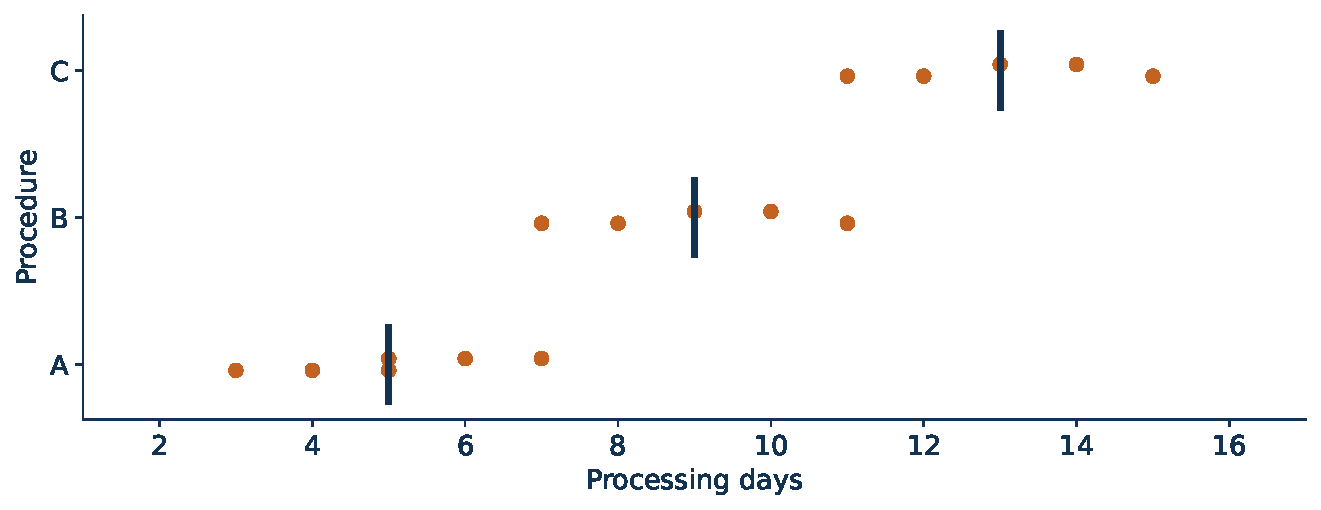
\includegraphics[width=.8\textwidth]{figures/groups_block2.pdf}\end{center}\small Constructed processing times: means 5, 9 and 13 days; six cases per group; each sample variance is 2 days$^2$. Vertical lines mark means.
\end{frame}
\begin{frame}{Ask about separation and spread}
\begin{block}{\href{https://silviasaliniunimi.github.io/data-analysis-tax-compliance/04-bivariate.html}{\textcolor{white}{E-tivity 4}}, section 5: 5 minutes}Increase the gap between means while holding within-group spread fixed. Then increase within-group spread while holding means fixed.\end{block}
\begin{itemize}\item Large mean differences relative to internal spread are easier to distinguish.\item A grand mean must weight groups by their sizes.\item A distribution plot can expose skewness, outliers and heterogeneity hidden by a mean.\end{itemize}
\end{frame}
\begin{frame}{Two groups: independent or paired?}
\begin{itemize}\item Independent procedures: use a two-sample comparison of means.\item Welch's t test estimates group variances separately.\item The pooled t test assumes a common variance.\item Before/after on the same cases: analyse paired differences.\end{itemize}
\begin{block}{Exact link under the matching classical model}With two independent groups and a common variance, one-way ANOVA has $F=t^2$ and the same p-value as the two-sided pooled t test.\end{block}
\end{frame}
\begin{frame}{ANOVA separates two sources of variation}
\[
SS_T=\sum_j\sum_i(x_{ij}-\bar x)^2=SS_B+SS_W,
\]
\[
SS_B=\sum_j n_j(\bar x_j-\bar x)^2,\qquad
SS_W=\sum_j\sum_i(x_{ij}-\bar x_j)^2.
\]
\begin{itemize}\item Between: weighted separation of group means from the grand mean.\item Within: deviations of observations from their own group means.\end{itemize}
For our groups: $SS_B=192$, $SS_W=30$, $SS_T=222$.
\end{frame}
\begin{frame}{The ANOVA table}
\begin{center}\begin{tabular}{lrrr}\toprule
Source & SS & df & MS\\\midrule
Between groups & 192 & $k-1=2$ & 96\\
Within groups & 30 & $n-k=15$ & 2\\
Total & 222 & $n-1=17$ & ---\\\bottomrule
\end{tabular}\end{center}
\[
F=\frac{MS_B}{MS_W}=\frac{96}{2}=48.
\]
Under the classical null model, compare this with $F_{2,15}$; p-value is the right-tail area.
\end{frame}
\begin{frame}{What does the global F test establish?}
\[
H_0:\mu_A=\mu_B=\mu_C,\qquad H_1:\text{not all means are equal}.
\]
Here $F(2,15)=48$, $p\approx3.03\times10^{-7}$.
\begin{itemize}\item Reject equal population means under the assumptions.\item This does not tell us that every pair differs.\item It does not establish that changing procedure caused the difference.\end{itemize}
\prompt{Which additional comparisons or design information would you need?}
\end{frame}
\begin{frame}{Effect size: eta-squared}
\[
\eta^2=\frac{SS_B}{SS_T}=\frac{192}{222}=.8649.
\]
About 86.5\% of observed total squared variation is associated with group membership in this deliberately separated example.
\begin{itemize}\item This is a descriptive variance proportion.\item It is not the probability that the test is correct.\item It is not a causal fraction of processing time.\end{itemize}
\prompt{Can a tiny between-group effect become significant in a sufficiently large sample?}
\end{frame}
\begin{frame}{Check the model and plan the follow-up}
\begin{itemize}\item Classical one-way ANOVA: independent observations, normal within-group errors and common population error variance.\item Use group and residual plots; independence depends on the study design.\item Unequal variances: consider Welch ANOVA.\item Pairwise follow-up: use justified contrasts or multiplicity-adjusted methods, such as Tukey under the classical model.\end{itemize}
Testing many pairs without adjustment inflates the chance of false positives.
\end{frame}
\begin{frame}{Two quantitative variables: start with a plot}
\begin{center}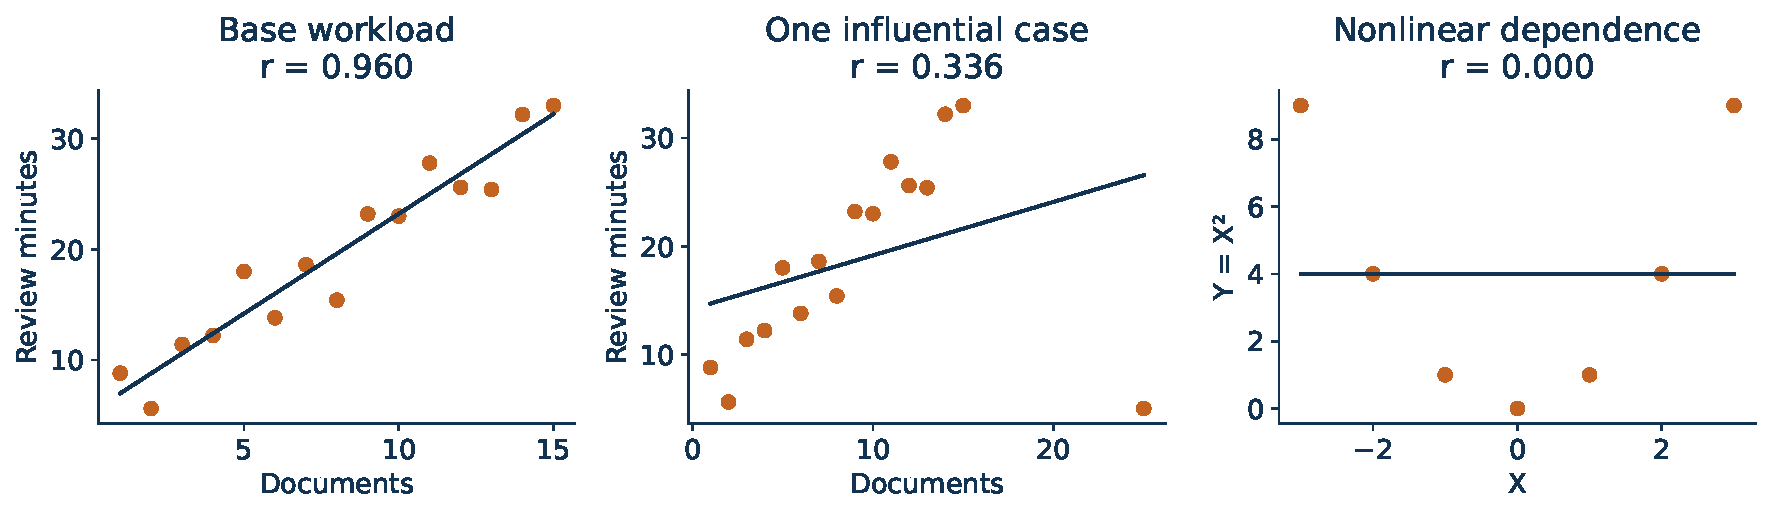
\includegraphics[width=.95\textwidth]{figures/scatter_block2.pdf}\end{center}\small A fitted line and r can change after one influential observation. Zero correlation can coexist with a deterministic nonlinear relationship.
\end{frame}
\begin{frame}{Covariance: matching and opposing deviations}
\[
s_{XY}=\frac1{n-1}\sum_i(x_i-\bar x)(y_i-\bar y).
\]
\begin{itemize}\item Both deviations positive or both negative: positive contribution.\item Opposite signs: negative contribution.\item Covariance units are the product of the two variables' units.\end{itemize}
\prompt{Would expressing review time in seconds rather than minutes change covariance?}
\end{frame}
\begin{frame}{Pearson correlation standardises covariance}
\[
r=\frac{s_{XY}}{s_Xs_Y}=\frac{\sum_i(x_i-\bar x)(y_i-\bar y)}{\sqrt{\sum_i(x_i-\bar x)^2\sum_i(y_i-\bar y)^2}}.
\]
\begin{itemize}\item $-1\le r\le1$, provided both variables vary.\item r describes the direction and strength of a \textbf{linear} association.\item It is symmetric in X and Y; it is not a slope.\item Population correlation $\rho$ and its sample estimate r are distinct.\end{itemize}
\end{frame}
\begin{frame}{The same r can hide different relationships}
\begin{center}\begin{tabular}{lrr}\toprule
Relationship & r & Slope\\\midrule
$Y=2X$ & 1 & 2\\
$Y=3X$ & 1 & 3\\
$Y=X^2$, symmetric $X=-3,\ldots,3$ & 0 & 0 (linear fit)\\\bottomrule
\end{tabular}\end{center}
\begin{itemize}\item Strength of a linear relationship is distinct from its size in units.\item Independence implies zero covariance when the relevant moments exist.\item Zero covariance/correlation does not generally imply independence.\end{itemize}
\end{frame}
\begin{frame}{Simpson: a headline worth checking}
\begin{block}{A misleading causal headline}``Reminders reduce compliance: 66\% versus 74\% on time.''\end{block}
\begin{center}\begin{tabular}{lrr}\toprule
Case complexity & Reminder & Standard\\\midrule
Simple & $18/20=90\%$ & $64/80=80\%$\\
Complex & $48/80=60\%$ & $10/20=50\%$\\\midrule
Total & $66/100=66\%$ & $74/100=74\%$\\\bottomrule
\end{tabular}\end{center}
\prompt{Both conditional comparisons favour the reminder group. How can the total reverse?}
\end{frame}
\begin{frame}{Different weights explain the reversal}
\begin{center}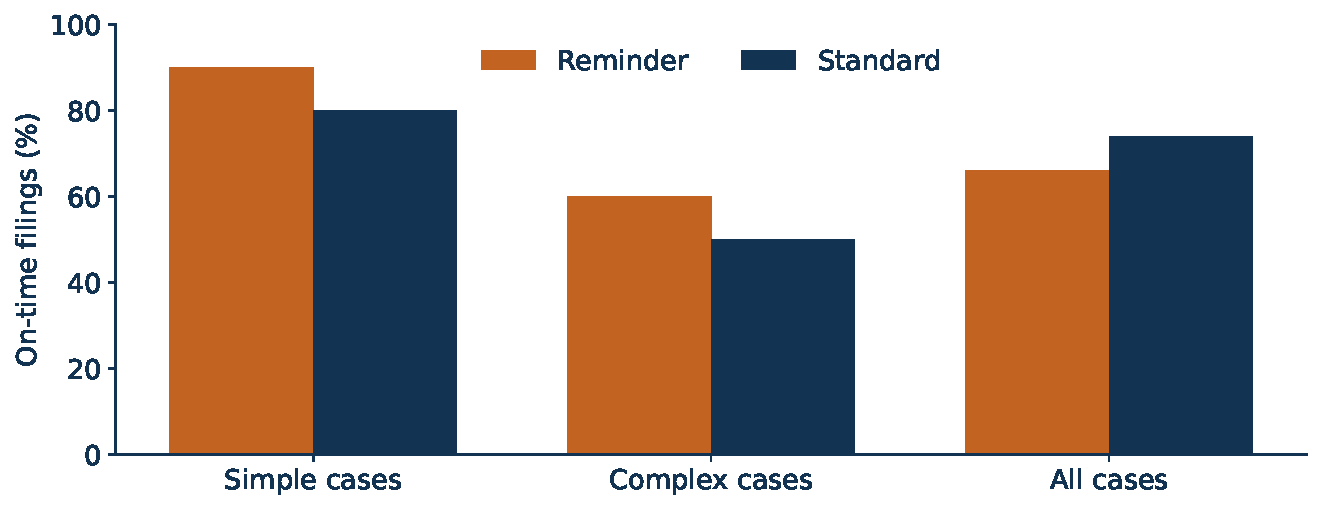
\includegraphics[width=.77\textwidth]{figures/simpson_block2.pdf}\end{center}\small Reminder: $.2(.9)+.8(.6)=.66$. Standard: $.8(.8)+.2(.5)=.74$. Reminder cases are much more concentrated in the complex stratum.
\end{frame}
\begin{frame}{Stratification does not automatically establish causation}
\begin{itemize}
\item Marginal and conditional associations can answer different questions.
\item Choose adjustment variables from substantive reasoning and the causal question.
\item Neither the aggregate table nor a reversal proves a policy effect.
\item Selection, timing, measurement and unobserved differences may remain.
\end{itemize}\prompt{Use the mixture sliders. Then rewrite the headline without asserting causation.}
\end{frame}
\begin{frame}{A complete bivariate comment}
\begin{itemize}
\item State the units, variables, question and target population.
\item Describe the table or plot and report the effect in meaningful terms.
\item Name the test and assumptions; interpret the p-value.
\item Report an effect size and a limitation on generalisation or causation.
\end{itemize}\prompt{Complete the 200--250 word e-tivity report and export your responses. Bring one question to the separate R lesson.}\source{Core lecture ends here. The remaining slides are optional reference/learning bridges.}
\end{frame}
\begin{frame}{Optional bridge: a fitted line has a direction}
\[
\widehat y=b_0+b_1x,\qquad b_1=\frac{s_{XY}}{s_X^2},\quad b_0=\bar y-b_1\bar x.
\]
OLS minimises $SSE=\sum_i(y_i-\widehat y_i)^2$, the squared vertical residuals.
For the base workload sample:
\[
\widehat{\text{minutes}}=5.1714+1.8036\times\text{documents}.
\]
An additional document is associated with about 1.804 more predicted minutes. This does not establish a causal effect.
\end{frame}
\begin{frame}{Optional bridge: fit, error and prediction}
For simple OLS with an intercept,
\[
R^2=1-\frac{SSE}{SST}=r^2=.9207,\qquad
SER=\sqrt{\frac{SSE}{n-2}}=2.4557\text{ minutes}.
\]
\begin{itemize}\item R$^2$ is a relative in-sample fit measure.\item SER describes residual spread in the units of Y.\item Neither is a substitute for evaluating prediction on new cases.\end{itemize}
We will return to training/test separation in supervised learning.
\end{frame}
\begin{frame}{Optional bridge: assumptions before regression inference}
\begin{itemize}
\item The conditional mean $E(Y\mid X)$ follows the specified linear form.
\item Errors are independent, with mean zero conditional on X.
\item Classical SEs assume constant conditional error variance.
\item Normal errors give exact small-sample t/F inference; X need not be marginally normal.
\end{itemize}Inspect residual patterns and influential points. A large R$^2$ does not validate these conditions.
\end{frame}
\begin{frame}{Optional bridge: slope uncertainty}
\[
SE(b_1)=\frac{SER}{\sqrt{\sum_i(x_i-\bar x)^2}}=.1468.
\]
With $n=15$, use $t_{.975,13}=2.1604$ for a 95\% interval:
\[
1.8036\pm2.1604(.1468)\approx[1.4865,2.1206]\text{ min/document}.
\]
For $H_0:\beta_1=0$, $t=b_1/SE(b_1)$, with 13 df. The p-value is about $1.57\times10^{-8}$ under the classical model.
The simple-regression global F statistic equals this slope-test $t^2$.
\end{frame}
\begin{frame}{Optional bridge: mean versus new-case intervals}
For a new document count $x_0$, define
\[
h_0=\frac1n+\frac{(x_0-\bar x)^2}{\sum_i(x_i-\bar x)^2}.
\]
\[
\text{Mean-response CI}:\quad \widehat y_0\pm t\,SER\sqrt{h_0},
\]
\[
\text{New-case prediction interval}:\quad \widehat y_0\pm t\,SER\sqrt{1+h_0}.
\]
The extra 1 represents individual variation. Both depend on the model; extrapolation adds unvalidated assumptions. Try $x_0=8$ and $20$; observed X ranges from 1 to 15.
\end{frame}
\begin{frame}{Reference: dependence is more than correlation}
For suitable finite moments:
\[
X\perp Y\ \Rightarrow\ E(Y\mid X)=E(Y)\ \Rightarrow\ \operatorname{Cov}(X,Y)=0.
\]
\begin{itemize}\item Mean independence as written is directional.\item The reverse implications do not hold in general.\item If the joint distribution is bivariate normal, zero correlation does imply independence.\end{itemize}
For i.i.d. bivariate normal data, the test of $H_0:\rho=0$ uses $t=r\sqrt{(n-2)/(1-r^2)}$ with $n-2$ df.
\end{frame}
\begin{frame}{R laboratory, Part B: bivariate analysis}
The supplied BES education materials provide examples of:
\begin{itemize}
\item Contingency tables: area and a dropout indicator.
\item Two groups: NEET percentages by dropout category.
\item Several groups: NEET percentages across geographical areas.
\item Quantitative pairs: tertiary education and cultural participation.
\end{itemize}
Regional percentages describe areas, not individual behaviour. Model-based tests require explicit assumptions when the dataset covers all regions.
\end{frame}
\begin{frame}{From bivariate analysis to supervised learning}
\begin{itemize}
\item A simple fitted line links the bivariate examples to prediction.
\item Multiple regression belongs to the supervised block, with validation and diagnostics.
\item A separate R session follows the theory of supervised learning.
\item The unsupervised block also pairs theory with examples in R.
\end{itemize}
\prompt{Which question concerns association in the observed data, and which concerns prediction for new cases?}
\end{frame}
